\chapter{Introduction}

\section{Motivation}

Most of today's popular relational databases use a \emph{Volcano}-style iterator model \cite{Graefe:1994:VEP:627290.627558} for query processing. In this processing model, each operator (say, a projection, selection, join, etc.) produces a stream of tuples. The output stream of another operator is consumed using a simple interface, consisting only of the functions \texttt{open()}, \texttt{next()} and \texttt{close()}.

\begin{figure}
\centering
\begin{subfigure}[b]{0.45\textwidth}
    \centering
    \begin{lstlisting}[language=SQL]
SELECT
  "c_nationkey",
  COUNT("c_custkey")
    AS "customers_in_debt"
FROM
  "customer"
  JOIN "nation"
    ON "c_nationkey" = "n_nationkey"
WHERE
  "c_acctbal" < 0 
GROUP BY
  "c_nationkey"
    \end{lstlisting}
    \caption{A simple SQL query}
    \label{fig:simple-query}
\end{subfigure}
\begin{subfigure}[b]{0.45\textwidth}
    \centering
    \begin{overpic}[scale=0.205]{introduction/volcano.pdf}
        \put(0, 0) {
            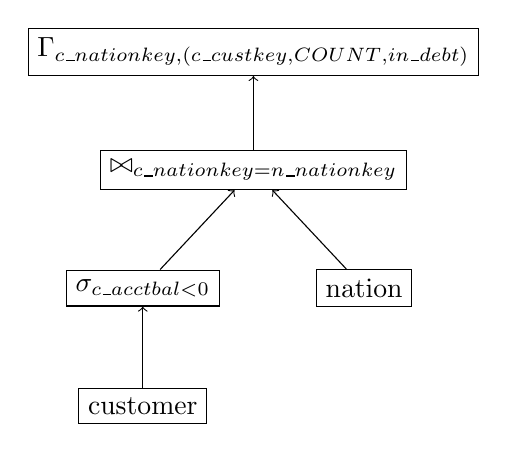
\begin{tikzpicture}[nodes={draw, rectangle}, sibling distance=80pt, <-]
                \node{$\Gamma_{\text{c\_nationkey}, (\text{c\_custkey}, \text{COUNT}, \text{in\_debt})}$}
                    child{node{$\bowtie_{\text{c\_nationkey} = \text{n\_nationkey}}$}
                        child{node{$\sigma_{\text{c\_acctbal} < 0}$}
                            child{node{customer}}}
                        child{node{nation}}};
            \end{tikzpicture}
        }
    \end{overpic}
    \caption{Evaluating \ref{fig:simple-query} using Volcano processing}
    \label{fig:volcano-processing}
\end{subfigure}
\\[5ex]
\begin{subfigure}[b]{0.45\textwidth}
    \centering
    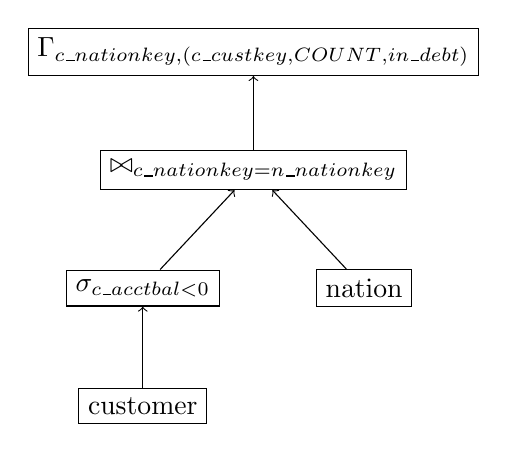
\begin{tikzpicture}[nodes={draw, rectangle}, sibling distance=80pt, <-]
        \node{$\Gamma_{\text{c\_nationkey}, (\text{c\_custkey}, \text{COUNT}, \text{in\_debt})}$}
            child{node{$\bowtie_{\text{c\_nationkey} = \text{n\_nationkey}}$}
                child{node{$\sigma_{\text{c\_acctbal} < 0}$}
                    child{node{customer}}}
                child{node{nation}}};
    \end{tikzpicture}
    \caption{Evaluating \ref{fig:simple-query} using bulk processing}
    \label{fig:bulk-processing}
\end{subfigure}
\begin{subfigure}[b]{0.45\textwidth}
    \centering
    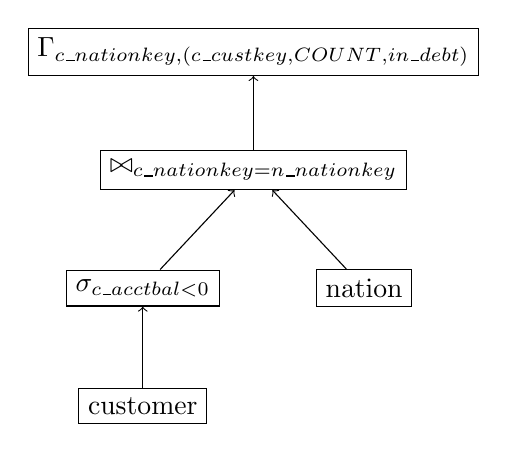
\begin{tikzpicture}[nodes={draw, rectangle}, sibling distance=80pt, <-]
        \node{$\Gamma_{\text{c\_nationkey}, (\text{c\_custkey}, \text{COUNT}, \text{in\_debt})}$}
            child{node{$\bowtie_{\text{c\_nationkey} = \text{n\_nationkey}}$}
                child{node{$\sigma_{\text{c\_acctbal} < 0}$}
                    child{node{customer}}}
                child{node{nation}}};
    \end{tikzpicture}
    \caption{Evaluating \ref{fig:simple-query} using code generation}
    \label{fig:code-generation}
\end{subfigure}
\caption{Approaches for improving query processing time}
\end{figure}

Whilst these databases benefit from a clean and flexible design which maximises maintainability and developer productivity, the Volcano-style processing model makes excessive use of function calls. For example, consider alone the \texttt{next()} call, which must be made for every tuple in the input, each intermediate result, and the final result. As main memory has grown, CPU costs now tend to be the query processing, and these function calls lead to frequent instruction mispredictions, and by extension control hazards, requiring CPU stalls which significantly degrade performance.

Database systems such as \emph{MonetDB} \cite{Boncz:2008:BMW:1409360.1409380} pioneered a bulk-processing approach, in which instead of considering one tuple at a time, entire columns are considered at a time. By doing so, the cost of calling the next operator is amortised over the number of tuples. However, this approach introduces a new cost: intermediate results must now be materialised. Whilst the iterator-model can pipeline most operators (that is, the output of one operator can be passed directly to the input of the next), this is no longer possible with the bulk-processing model, which must make all resulting tuples accessible to the next operator to process at once. This often results in memory bandwidth constraining performance.

In an attempt to solve this, a new query engine, \emph{X100} \cite{DBLP:conf/cidr/BonczZN05} (which later evolved into VectorWise), was built for MonetDB, which processes smaller (say 1000-value) vectors, which form chunks of columns. These vectors can fit in the CPU cache, and can be pipelined to avoid expensive materialisation.

More recently, the \emph{HyPer} in-memory database system \cite{Neumann:2011:ECE:2002938.2002940} was shown to significantly outperform MonetDB and VectorWise in most cases, by using LLVM to compile queries into machine code with better locality and a more predictable branch layout. In this approach, chains of operators which can be pipelined (i.e. chains that do not require materialisation) are identified, and each of these fragments is compiled separately into machine code. This reverses the direction of data-flow control: instead of each operator asking its input for tuples, each fragment of code processes the data and makes it available to the next fragment. Operators within each fragment leave tuples inside the CPU registers and so are extremely cheap, whilst pipeline-breaking operators (at the edge of fragments) would have required materialisation anyway, so there is no significant performance implication for them.

\emph{Voodoo} \cite{Pirk:2016:VVA:3007328.3007336} is a vector algebra which can be used as an intermediate representation between a database query and a code implementation, similar to what HyPer might produce. Voodoo allows the often data and hardware dependant kind of optimisations used in systems such as HyPer to be expressed in a portable way, and is designed to be \emph{tunable}, that is, it is able to express very simply most optimisations for in-memory query processing. It has been shown to generate highly-efficient OpenCL code to run on GPUs, outperforming existing state-of-the-art in-memory query processors for many queries.

Whilst benchmarks have shown that using Voodoo allows some of the fastest query processing times out of any modern approach, it was not really available in a form that made it easy to use:

\begin{enumerate}
    \item The existing Voodoo implementation was used as a replacement back-end for MonetDB. However the components to convert a query to a MonetDB plan and a MonetDB plan to Voodoo algebra remained mostly separate to the Voodoo kernel (code generator) itself, so there was no way to run queries, apart from TPC-H benchmarking queries whose plans were hard-coded into the driver program.
    \item The code generation itself was done by concatenating strings which formed the OpenCL program. This approach resulted in complex and fragile code, which was very difficult to extend. Importantly, once code had been written to the string, it became extremely difficult to change or move.
    \item Certain parts of the code also suffered from particularly sparse documentation, and several bugs which were identified during this project.
\end{enumerate}

\section{Objectives}

Main goal: make this usable for researchers: provide a front-end to what was just a benchmarking application, improve code generation...

1. Build a front-end to get SQL -> Logical plan -> Vooodoo for arbitrary schema, query.

2. Generate code using AST, to improve readability of generated code, and ease of implementation.

\section{Achievements}

Use \url{https://docs.google.com/document/d/1tCYCOFDeL8E3USIOunRNrqh6ekP_-kAQVHMrNJ4jk04} for achievments. Try to back everything up in a quantifiable way...

% We have developed a front-end for the Voodoo kernel, which allows for arbitrary queries to be run through a single program. In addition to this, we have provided a CI setup which demonstrates a provably correct setup for building the database system. We claim that this has made Voodoo much more accessible to researchers, who will be able to set up and begin to use Voodoo much more easily. They can connect to Voodoo using JDBC, and view the logical plan, Voodoo algebra and OpenCL code for a query, as well as the results of its execution.

% Furthermore, we have written a new implementation for the Voodoo kernel that uses an AST to generate OpenCL code. This implementation is less fragile and complex than the existing string-based implementation. We claim that it produces simpler code with performance roughly comparable to the existing implementation in most cases. We believe that it also significantly improves the extensibility of the Voodoo kernel.

1. Document and formalise installation...

1a. Contribute bugfixes required to get code to compile and run, update documentation

1b. Provide a dockerfile that prescribes the required setup

1c. Introduce CI that ensures the project can always build

2. Develop Calcite adapter that supports these SQL queries...

2a. Support arbitrary schemas with these types compared to before...

2b. Support arbitrary queries using these logical operators compared to before...

2c. Support rule-based logical optimisations using Calcite...

2d. Support enumerable operators using Calcite...

2e. Support integration with C++ printer implementation...

2f. Support integration with C++ AST implementation, by extending API...

2g. Provide a JDBC connection through Calcite

(2h. Provide a front-end that demonstrates the full process).

3. Develop a Clang-AST based implementation of Voodoo API.

3a. Support these Voodoo operators compared to before...

3b. Improve quality of implementation code as measured by this metric...

3c. Improve quality of generated code as measured by this metric...

3d. Improve ease-of-use as demonstrated by example (cross?), by providing AST components...

3e. Support future extension to C-like languages such as CUDA through generic processing class...
